\documentclass[letterpaper]{article}

% AAAI-27 author-kit baseline. Keep submission mode until the anonymous-review
% process is complete.
\usepackage[submission]{aaai2027}
\usepackage[hyphens]{url}
\usepackage{graphicx}
\urlstyle{rm}
\def\UrlFont{\rm}
\usepackage{natbib}
\usepackage{caption}
\usepackage{booktabs}
\frenchspacing
\pdfinfo{/TemplateVersion (2027.1)}
\usepackage{amsmath,amssymb}
\usepackage{tikz}
\usetikzlibrary{arrows.meta,positioning}
\setcounter{secnumdepth}{2}
\usepackage{tabularx}
\usepackage{xcolor}
\usepackage{makecell}
\usepackage{todonotes}
\usepackage{pdfpages}
\usepackage{fvextra}

\newcommand{\fixme}[3]{%
  \todo[inline,color=#3]{\textbf{#1:} #2}%
}
\newcommand{\dan}[1]{\fixme{Dan}{#1}{orange!45}}
\newcommand{\kobi}[1]{\fixme{Kobi}{#1}{cyan!20}}

% Working title retained after the P9 whole-paper audit. Final human approval
% remains TODO-HUMAN G-HUM-01.
\title{CliniCause: Constructing Clinically Grounded Observational Testbeds for Causal Analysis}
\affiliations{}

\begin{document}
\maketitle


\begin{abstract}
Causal estimators are commonly evaluated using synthetic, semi-synthetic, or
experimentally anchored benchmarks whose ground truth depends on
researcher-specified data-generating or sampling mechanisms. We introduce
\emph{CliniCause}, a complementary framework for constructing observational
causal-analysis testbeds without generating patient records, exposure
assignments, or outcomes. CliniCause uses literature-grounded LLM elicitation
to define clinically motivated proxy exposures and a causal graph, then
instantiates this representation on source-observed longitudinal ICU records
from MIMIC-III and PhysioNet 2012. We evaluate the resulting resources through
proxy recoverability, mortality prediction, cross-estimator agreement,
permutation tests, omitted-variable sensitivity analysis, and comparison with
clinical literature. The results show broad predictive and cross-estimator
consistency alongside meaningful sensitivity to modest unobserved confounding,
demonstrating the value of real observational testbeds for exposing estimator
fragility that controlled benchmarks may not reveal.
\end{abstract}
% Causal estimators are commonly evaluated on synthetic, semi-synthetic, or
% experimentally anchored benchmarks. These resources provide answer keys, but
% performance remains conditional on researcher-specified data-generating,
% sampling, or data-fusion mechanisms. We introduce \emph{CliniCause}, a
% representation-centered pipeline for constructing causal-analysis testbeds from
% source-observed data without simulating patients, exposure assignments, or
% outcomes. Literature-grounded knowledge, elicited with an LLM and inspected by
% the authors, defines proxy exposures and a causal graph from irregular clinical
% time series. Deterministic rules and four temporal models produce patient-level
% exposures through a fixed majority vote. Applied to MIMIC-III and PhysioNet 2012, CliniCause produces two evidence-tracked
% resources containing 26,845 and 7,993 records and nine and ten proxy exposures,
% respectively. Archived held-out results achieve macro AUROC values of
% 0.867--0.918 and AUPRC values of 0.823--0.905 for proxy recovery.
% CausalForestDML and LinearDML agree in effect direction across all 19
% dataset--exposure comparisons, while CausalPFN agrees in 18 of 19. Comparisons
% with published clinical evidence identify both plausible patterns and a notable
% discrepancy for shock. CliniCause does not provide causal ground truth; it
% provides auditable infrastructure for evaluating causal methods under
% source-observed real-world processes.
\section{Introduction}

Causal inference asks how outcomes would change under alternative actions,
rather than only which outcomes can be predicted. This distinction is central
to medicine and public policy: an accurate forecast may identify who is at
risk, but it does not establish which action is needed.
Modern causal machine-learning methods support flexible adjustment and
heterogeneous-effect estimation
\cite{chernozhukov2018dml,wager2018causalforest,shalit2017ite,
louizos2017cevae}, but evaluating them is unusually difficult. For each
individual, the counterfactual outcome needed to score an estimated effect is
unobserved.

Because observational data do not reveal counterfactual outcomes, they do not
provide a direct answer key for evaluating causal estimators. They also leave
the true treatment-assignment process and the extent of unmeasured confounding
unknown. The safest experimental sandbox is therefore fully synthetic data: the evaluator specifies the covariates, treatment assignment, potential outcomes, confounding, overlap, and effect heterogeneity. Assumptions such as
ignorability or positivity can be satisfied, violated, or gradually stressed
under complete control, while the true causal effect remains known.


\begin{figure*}[t]
\centering
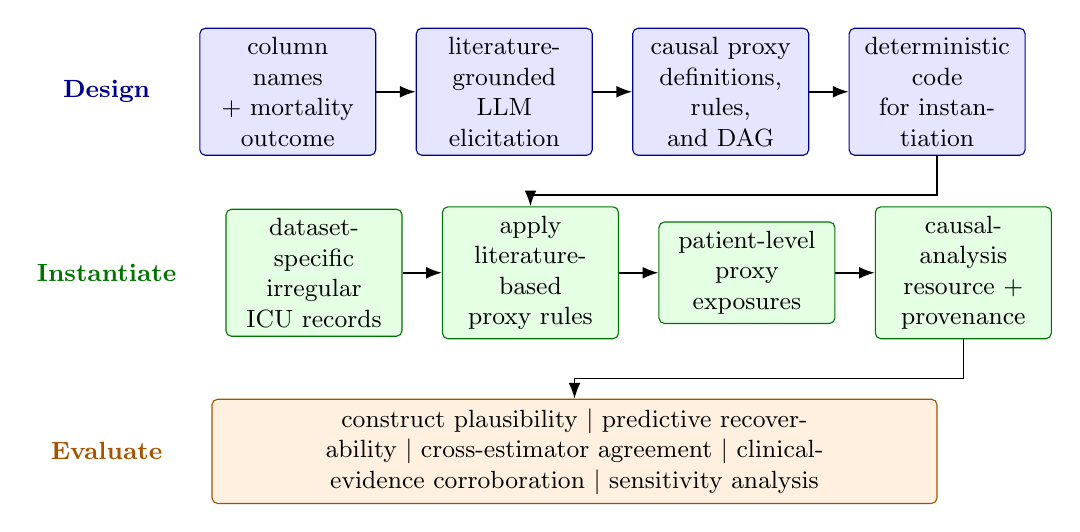
\begin{tikzpicture}[
  node distance=4mm and 5mm,
  box/.style={
    draw,
    rounded corners=2pt,
    align=center,
    minimum height=8mm,
    text width=0.165\textwidth,
    font=\small
  },
  designbox/.style={
    box,
    fill=blue!10,
    draw=blue!55!black
  },
  instantiatebox/.style={
    box,
    fill=green!10,
    draw=green!45!black
  },
  evaluatebox/.style={
    box,
    fill=orange!12,
    draw=orange!65!black
  },
  arr/.style={
    -{Latex[length=2mm]},
    line width=0.6pt
  },
  stage/.style={
    font=\small\bfseries,
    anchor=east
  }
]

% Design stage
\node[stage, text=blue!55!black] (s1) {Design};
\node[designbox, right=of s1] (schema)
  {column names\\+\ mortality outcome};
\node[designbox, right=of schema] (llm)
  {literature-grounded\\LLM elicitation};
\node[designbox, right=of llm] (constructs)
  {causal proxy definitions,\\rules, and DAG};
\node[designbox, right=of constructs] (encode)
  {deterministic code\\for instantiation};

% Instantiation stage
\node[stage, below=18mm of s1, text=green!45!black] (s2)
  {Instantiate};
\node[instantiatebox, right=of s2] (records)
  {dataset-specific irregular\\ICU records};
\node[instantiatebox, right=of records] (rules)
  {apply literature-based\\proxy rules};
\node[instantiatebox, right=of rules] (proxies)
  {patient-level\\proxy exposures};
\node[instantiatebox, right=of proxies] (resource)
  {causal-analysis\\resource + provenance};

% Evaluation stage
\node[stage, below=18mm of s2, text=orange!65!black] (s3)
  {Evaluate};
\node[evaluatebox, right=of s3, text width=0.74\textwidth] (eval)
  {construct plausibility \(\mid\) predictive recoverability \(\mid\)
   cross-estimator agreement \(\mid\) clinical-evidence corroboration
   \(\mid\) sensitivity analysis};

% Within-stage arrows
\draw[arr] (schema) -- (llm);
\draw[arr] (llm) -- (constructs);
\draw[arr] (constructs) -- (encode);

\draw[arr] (records) -- (rules);
\draw[arr] (rules) -- (proxies);
\draw[arr] (proxies) -- (resource);

% Between-stage arrows
\draw[arr] (encode.south) -- ++(0,-5mm) -| (rules.north);
\draw[arr] (resource.south) -- ++(0,-5mm) -| (eval.north);

\end{tikzpicture}

\caption{The three stages of CliniCause. Schema-level clinical knowledge is
used to define causal proxy states, literature-based rules, and a DAG.
Deterministic code instantiates this representation on dataset-specific ICU
records, after which the resulting causal-analysis resources are evaluated.
Critically, the LLM receives schema information rather than patient-level records.}
\label{fig:pipeline}
\end{figure*}



That control creates an important limitation. The evaluator determines not only
the answer but also the difficulty of recovering it. A method may perform well
because its assumptions align with the selected assignment model, response
surface, confounding structure, or overlap regime. Semi-synthetic benchmarks
move closer to observed data by retaining empirical covariates while simulating
treatment assignments, potential outcomes, or both. RCT-derived and
empirically anchored designs preserve still more of the observed system, but
continue to obtain an answer key through researcher-controlled sampling,
comparison, or generation mechanisms. Across this spectrum, greater control
makes accuracy measurable, while greater observational fidelity makes the
causal target less knowable.


Several widely used causal-ML resources illustrate this spectrum of constructed
evaluation. IHDP retains empirical covariates while simulating outcomes, whereas
ACIC uses empirical covariates within diverse simulated treatment and outcome
mechanisms; Dragonnet, for example, evaluates 101 retained datasets drawn from
63 ACIC 2018 data-generating settings
\cite{shalit2017ite,shi2019dragonnet}. Influence-function validation similarly
compares models across 77 semi-synthetic competition datasets sharing one
empirical feature source but using distinct simulated assignments and outcomes
\cite{alaa2019validating}. More empirically grounded designs retain additional
observed components: observational sampling from randomized trials preserves
real trial variables but induces confounding through researcher-specified
selection \cite{gentzel2021experimental}; Jobs/LaLonde combines experimental
treated subjects with external non-experimental controls, making comparability
depend on population-selection and harmonization choices; and Credence learns
from an empirical distribution, but generates data under user-specified effects
and confounding \cite{parikh2022validating}. These designs are increasingly
sophisticated and provide valuable causal answer keys. Nevertheless, measurable
accuracy still depends on an experimental anchor or a researcher-constructed
causal, sampling, or comparison mechanism. They therefore cannot by themselves
show how estimators behave when exposure prevalence, missingness, support, and measurement processes arise from routine practice rather than from the
evaluation design.


\subsection*{Our Contribution.}
We propose shifting researcher intervention in causal evaluation from the
data-generating process to the \emph{representation layer}. Consider estimating
the effect of ICU shock on mortality. A synthetic benchmark specifies how shock
is assigned and how mortality is generated, thereby providing a known answer
under researcher-selected mechanisms. Our alternative preserves the
source-observed measurements, clinical practice, missingness, empirical
support, and mortality, while explicitly defining how those records become
exposures, covariates, cohorts, and adjustment assumptions.

We instantiate this approach through \emph{CliniCause}, an evidence-tracked
pipeline applied to MIMIC-III and PhysioNet 2012
\cite{johnson2016mimiciii,silva2012physionet}. ChatGPT was given the available
column names and mortality outcome, but not patient records, distributions, or
estimated effects. It was instructed to identify literature-supported clinical
states treated as causal determinants of mortality, operationalize them using
measurement cutoffs and temporal rules, and propose a DAG relating the states,
observed variables, measurement processes, and mortality. Each proposed proxy,
cutoff, and edge was required to include a clinical rationale and supporting
source, making the representation inspectable and replaceable. The LLM thus served as a knowledge-elicitation assistant, not as a source of
causal ground truth or a mechanism for generating ground truth from the
observational data.

Applied to 26,845 MIMIC-III and 7,993 PhysioNet records, CliniCause produced
resources with nine and ten proxy exposures, respectively, including renal and
hepatic dysfunction, shock, respiratory failure, cardiac strain, and
sepsis-related burden. 

Although the represented clinical states were selected because the medical literature treats them as causal determinants of mortality, this construct-level evidence does not establish causal identification in these particular datasets.
The operational rules, cutoffs, temporal aggregation, cohort definitions, and
DAG-based adjustment sets may still introduce measurement error, selection
bias, model misspecification, or unmeasured confounding. Because the resulting
resources therefore have no known causal answer, we evaluate their construction
through converging evidence. Informal ICU-physician consultation assesses construct
plausibility; temporal models (STraTS, GRU, GRU-D, and TCN) tested proxy recoverability from the irregular time
series using three-fold cross-validation; three causal
estimators assess effect-pattern stability; and published clinical evidence
provides external directional and scale comparisons. Across 19 prespecified
dataset--exposure comparisons, CausalForestDML and LinearDML agreed in direction
in all 19, while CausalPFN agreed in 18. Comparison with the clinical literature corroborated most estimated patterns
while also identifying several discrepancies for further investigation. 




% In this paper, we propose a pivot in where researchers intervene when
% constructing causal-evaluation resources. Before defining this paradigm
% formally, consider a running ICU example in which the goal is to estimate how a
% shock state affects in-hospital mortality. The raw record does not contain a
% single, ready-made shock variable. Instead, it contains an irregular sequence
% of blood-pressure measurements, lactate tests, urine-output observations, and
% vasopressor administrations, followed by a source-observed mortality outcome.

% A fully synthetic benchmark could generate the patients, assign shock according
% to a researcher-specified probability, and simulate mortality under shock and
% no shock. A semi-synthetic benchmark could retain observed patient covariates
% while simulating the shock assignment, mortality outcomes, or both. Either
% construction provides a known causal answer, but both the answer and the
% difficulty of recovering it depend on researcher-selected mechanisms.



% We propose shifting this intervention from the data-generating process to the
% \emph{representation layer}. In the running example, the evaluator preserves
% the shock-related measurements, clinical practice patterns, missingness,
% empirical support, and mortality recorded during routine care. The evaluator
% intervenes by specifying which measurements and temporal rules define the shock
% exposure, which patients enter the cohort, which variables serve as covariates
% and outcomes, and which causal relationships determine adjustment. 

% Crucially,
% these choices are knowledge-driven rather than learned from exposure--outcome
% associations in the evaluation data. Clinical experts, published evidence, or
% externally elicited domain knowledge specify, for example, that hypotension,
% elevated lactate, low urine output, and vasopressor use constitute evidence of
% shock; the dataset is not searched for the definition that produces the
% strongest mortality effect. Patient records are used to instantiate this
% prespecified representation. This separation reduces outcome leakage and
% post-hoc selection while making every threshold, temporal rule, cohort
% restriction, and graph edge an explicit knowledge claim that can be inspected,
% challenged, and replaced.

% LLMs make this knowledge-driven construction increasingly scalable. Their broad
% clinical knowledge can support structured elicitation of candidate constructs
% and relationships
% \cite{singhal_et_al_2023_llm_clinical_knowledge}, while their reliability
% limitations require that every proposal remain auditable and subordinate to
% external evidence and expert review
% \cite{darvariu_et_al_2024_llm_causal_graph_priors}. The LLM therefore serves as
% a design assistant rather than a source of causal ground truth: it helps make
% the proposed representation explicit but does not process patient records,
% generate exposures or outcomes, or select definitions according to their
% estimated effects.

% The running example reflects the real setting studied in this paper. We
% instantiate the representation-centered paradigm through \emph{CliniCause}, an
% evidence-tracked pipeline applied to longitudinal ICU records from MIMIC-III
% and PhysioNet 2012 \cite{johnson2016mimiciii,silva2012physionet}.

% CliniCause uses ChatGPT through its desktop interface as a knowledge-elicitation
% assistant at the representation stage. ChatGPT was given the names of the
% columns available in the ICU time series and the target outcome, but not the
% patient-level records, variable distributions, exposure prevalences, causal
% estimates, or access to the environment containing MIMIC-III and PhysioNet.
% Drawing on clinical literature available through its pretrained knowledge and
% online search, ChatGPT was explicitly instructed to identify clinically
% meaningful states that the medical literature treats as causal determinants of
% mortality, rather than merely predictive correlates. It was then asked to
% operationalize these states as categorical proxy exposures using
% literature-grounded measurement cutoffs and temporal rules, and to construct a
% DAG relating the proxies, observed covariates, measurement processes, and
% mortality. Thus, every proposed proxy, cutoff, and DAG edge is accompanied by a clinical
% rationale and supporting literature source, making each knowledge claim
% traceable and open to verification.


% Applied to 26,845 MIMIC-III and 7,993 PhysioNet records,
% it produced resources with nine and ten admitted proxy exposures, respectively, including
% renal and hepatic dysfunction, shock, respiratory failure, cardiac strain, and
% sepsis-related burden. 

% By preserving the naturally occurring measurement, exposure, support, and
% outcome processes, CliniCause gives up the known answer provided by controlled
% benchmarks. Its credibility must therefore come from converging evidence rather
% than comparison with causal ground truth. We examine the resources along four
% complementary axes: whether the candidate exposures and graph assumptions are
% clinically plausible; whether the rule-derived constructs are recoverable from
% the underlying measurements; whether distinct causal estimators agree once the
% representation is fixed; and whether the estimated directions corroborate
% mortality relationships reported in independent clinical studies. Together,
% these checks assess whether CliniCause provides a convincing and useful
% observational causal testbed, without treating its proxies as literal
% interventions, its DAG as known to be correct, or its estimated effects as
% ground-truth causal answers.

% We evaluate the resulting resources along each of the four proposed axes.
% Informal consultations with ICU physicians provided formative feedback on the
% clinical plausibility of the proxies and graph assumptions, while predictive
% experiments assessed whether the rule-derived proxies could be recovered from
% the underlying measurements. Across 19 prespecified dataset--exposure
% comparisons, CausalForestDML and LinearDML agreed in direction in all 19, and
% CausalPFN agreed in 18; PhysioNet shock was the sole exception. Finally,
% comparison with published mortality gradients supported the renal, hepatic,
% cardiac, inflammation/sepsis, and global-severity directions, while identifying
% shock and PhysioNet coagulation/hematologic dysfunction as clinically
% discordant cases requiring further review
% (Table~\ref{tab:clinical-corroboration}). The physician consultations were
% informal rather than structured clinical adjudication, and the combined checks
% provide converging evidence rather than causal ground truth.

Our contributions, illustrated in Figure \ref{fig:pipeline}, can be summarized as follows:
\begin{enumerate}
    \item An evidence-tracked pipeline that converts irregular clinical records
    into explicit causal-analysis representations while preserving observed
    patient, support, and outcome processes;

    \item Two resources derived from MIMIC-III and PhysioNet 2012,
    containing 19 clinically motivated proxy-exposure analyses with inspectable
    cohort, graph, adjustment, and provenance assumptions; and
\item An evaluation framework based on construct plausibility, proxy
recoverability, cross-estimator agreement, permutation checks,
omitted-variable sensitivity analysis, and clinical-literature corroboration.
Its application shows that otherwise concordant double machine learning (DML)
estimates can remain fragile to modest unobserved confounding, demonstrating the value of the proposed resources for exposing weaknesses that agreement alone would conceal.
\end{enumerate}


% \begin{table*}[t]
% \centering
% \caption{Clinical-literature corroboration of selected original-cohort CATE
% estimates. Values are mean estimated changes in in-hospital mortality
% probability, in percentage points, for CausalForestDML (F), LinearDML (L), and
% CausalPFN (P). Literature findings provide directional and clinical-plausibility
% comparators, not ground-truth causal effects or direct calibration targets.}
% \label{tab:clinical-corroboration}
% \scriptsize
% \setlength{\tabcolsep}{3pt}
% \begin{tabular}{p{1.15in}p{1.35in}p{1.35in}p{3.0in}}
% \toprule
% \textbf{Proxy variable} &
% \textbf{MIMIC-III CATE (pp)} &
% \textbf{PhysioNet CATE (pp)} &
% \textbf{Clinical literature comparator and interpretation} \\
% \midrule

% Renal dysfunction / AKI &
% F: $+9.1$; L: $+8.9$; P: $+8.7$ &
% F: $+12.0$; L: $+9.1$; P: $+11.1$ &
% KDIGO defines AKI using creatinine and urine-output changes. AKI-EPI reports a
% stage-dependent mortality gradient, reaching an adjusted mortality OR of 6.884
% for stage 3; a septic-ICU cohort attributes approximately 16.8 percentage
% points of 30-day mortality to stage 3 AKI. The positive CATE direction and
% rough magnitude are clinically plausible, conditional on the proxy capturing
% moderate or severe AKI. \\

% Hepatic dysfunction / bilirubin &
% F: $+9.8$; L: $+8.3$; P: $+9.7$\textsuperscript{a} &
% F: $+9.1$; L: $+6.0$; P: $+10.7$ &
% ICU studies report higher mortality with elevated bilirubin: 30\% versus 21\%
% for bilirubin above 1 mg/dL, and 31.9\% versus 17.0\% for bilirubin at least
% 2 mg/dL in MIMIC-III. The positive $+6$ to $+11$ pp estimates are directionally
% and approximately quantitatively consistent. \\

% Cardiac strain / injury &
% F: $+22.0$; L: $+18.8$; P: $+25.9$ &
% F: $+11.2$; L: $+12.2$; P: $+11.9$ &
% A review of ICU troponin studies reports an adjusted mortality OR of 2.5 for
% elevated troponin; a sepsis meta-analysis reports mortality HR 1.57. The
% positive direction is supported, although the literature does not establish
% that cardiac strain should be the highest-ranked isolated causal pathway,
% particularly in MIMIC-III. \\

% Inflammation / sepsis burden &
% F: $+16.1$; L: $+16.1$; P: $+14.9$ &
% F: $+7.2$; L: $+7.1$; P: $+6.7$ &
% Sepsis-3 associates infection-related organ dysfunction with in-hospital
% mortality exceeding 10\%. The positive estimates are clinically plausible, but
% the large MIMIC-III estimate may indicate that the proxy captures organ
% dysfunction or measurement intensity in addition to inflammation
% \cite{singer_2016_sepsis3}. \\

% Global severity &
% F: $+6.2$; L: $+8.0$; P: $+7.3$ &
% F: $+10.8$; L: $+10.7$; P: $+10.5$ &
% SOFA was developed to describe organ dysfunction and failure, and increases in
% SOFA are strongly associated with mortality. The consistently positive
% estimates, particularly the approximately $+11$ pp PhysioNet estimates, are
% directionally plausible
% \cite{vincent_et_al_1996_sofa,singer_2016_sepsis3}. \\

% Shock &
% F: $+2.1$; L: $+2.1$; P: $+3.2$ &
% F: $-1.4$; L: $-2.7$; P: $+0.4$ &
% Sepsis-3 septic shock requires vasopressors and lactate above 2 mmol/L after
% resuscitation and is associated with hospital mortality above 40\%. The small
% MIMIC-III estimates and negative or near-zero PhysioNet estimates are
% \emph{not} clinically aligned with a total shock effect. This is an explicit
% red flag for proxy construction, temporal definition, mediator adjustment, or
% available treatment information \cite{singer_2016_sepsis3}. \\

% Coagulation / hematologic dysfunction &
% \multicolumn{1}{c}{--\textsuperscript{b}} &
% F: $+1.1$; L: $+0.4$; P: $+2.5$ &
% PLOT-ICU reports 90-day mortality of 34.6\% among patients with
% thrombocytopenia versus 19.3\% without it, rising to approximately 51--52\% in
% severe cases. The near-zero PhysioNet estimates are substantially weaker than
% this clinical gradient and constitute a second explicit proxy-validation
% red flag. \\

% \bottomrule
% \multicolumn{4}{p{6.95in}}{\footnotesize
% \textsuperscript{a} The MIMIC-III variable combines hepatic and coagulation
% dysfunction and is therefore not directly equivalent to the PhysioNet hepatic
% proxy.
% \textsuperscript{b} MIMIC-III has no separate coagulation/hematologic proxy;
% its mixed hepatic/coagulation variable cannot independently corroborate this
% clinical construct.
% F = CausalForestDML; L = LinearDML; P = CausalPFN; pp = percentage points.
% CausalPFN is exploratory and lacks the downstream diagnostics available for
% the two DML estimators.}
% \end{tabular}
% \end{table*}
\section{Related Work}

\paragraph{Clinical representation.}
Electronic phenotyping converts heterogeneous health records into computable
states using expert rules and learned models
\cite{banda_2018_electronic_phenotyping,ratner_et_al_2020_snorkel}.
GRU-D models informative missingness, while STraTS represents irregular
observations as time--variable--value events
\cite{che2018grud,tipirneni2022strats}. CliniCause differs by first eliciting
clinically and causally motivated proxy states and operational rules, and then
using temporal models to test their recoverability.

\paragraph{LLMs and causal knowledge.}
Medical LLMs encode substantial clinical knowledge but require verification
\cite{singhal_et_al_2023_llm_clinical_knowledge}. Prior work uses LLMs, clinical
literature, or observational associations to construct causal graphs, while
evaluations identify sensitivity to memorization and prompting
\cite{roy2025causalllm,feng2025reliability,
nordon2019medicalcausalgraphs}. CliniCause withholds patient records from the
LLM and instead uses schema-level information to elicit literature-grounded
proxy definitions, cutoffs, temporal rules, and their DAG.

\paragraph{Causal estimation and evaluation.}
Double machine learning and causal forests support flexible nuisance estimation
and heterogeneous effects
\cite{chernozhukov2018dml,wager2018causalforest,athey2019grf}, while
CausalPFN amortizes estimation across simulated data-generating processes
\cite{balazadeh2025causalpfn}. Existing evaluations use semi-synthetic,
RCT-derived, or empirically anchored benchmarks, including IHDP, ACIC,
Jobs/LaLonde, OSRCT, and Credence
\cite{alaa2019validating,gentzel2021experimental,
parikh2022validating}. These provide experimental or constructed answer keys;
CliniCause instead evaluates estimators under a knowledge-grounded
representation of source-observed clinical data.

\paragraph{Observational clinical causality and positioning.}
Causal EHR studies require explicit cohorts, exposures, outcomes, time zero,
and adjustment assumptions
\cite{hernan_robins_2016_target_trial,
hernan_taubman_2008_well_defined_interventions,bica_2021_individualized_treatment_effects_ehr_ml}.
Such representations are usually reconstructed for one clinical question.
CliniCause packages multiple clinically motivated exposures, proxy rules, DAGs,
adjustment sets, and provenance within a shared resource. To our knowledge,
prior work has not combined schema-only LLM knowledge elicitation,
deterministic instantiation on longitudinal records, and evaluation through
proxy recoverability, estimator agreement, and clinical-literature
corroboration.


\section{Methodology}

\begin{figure*}[t]
  \centering
  
\includegraphics[width=0.89\textwidth]{figures/figure3_shock_proxy_example.png}
  \caption{Example of ChatGPT-assisted, knowledge-driven proxy construction for
the shock exposure. Five binary clinical indicators
(\(H_i,V_i,P_i,O_i,A_i\)) are derived from the corresponding patient time
series and combined by an explicit deterministic rule to produce the
patient-level proxy \(Z_i^{\mathrm{shock}}\). ChatGPT proposes candidate
indicators, cutoffs, and combination logic at design time; the authors inspect
and encode the accepted specification.}
  \label{fig:shock-example}
\end{figure*}

In this section, we describe the CliniCause construction pipeline summarized in
Figure~\ref{fig:pipeline}: resource definition, knowledge-driven proxy and graph
design, patient-level instantiation, and provenance tracking. The subsequent
clinical-evidence validation is described in detail in
Section~\ref{sec:ClinicalEvidenceCorrob}.


\subsection{Clinical Setting and Resource Contract}

Let \(d\in\{\mathrm{MIMIC},\mathrm{PhysioNet}\}\) index the source database and
let
\[
\mathcal{I}_d=\{1,\ldots,N_d\}
\]
denote its set of analysis records. An analysis record is an ICU stay or source
time-series record, not necessarily a unique patient. For record
\(i\in\mathcal{I}_d\), the irregular clinical observations are
\[
\mathcal{X}^{(d)}_i
  =\{(t_{ij},v_{ij},x_{ij})\}_{j=1}^{n_i},
\]
where \(t_{ij}\), \(v_{ij}\), and \(x_{ij}\) denote the observation time,
measured variable, and recorded value. A linked record-level view supplies the
canonical identifier \(\mathrm{id}^{(d)}_i\), baseline covariates
\(\mathbf{C}^{(d)}_i\), and source-observed in-hospital mortality outcome
\(Y^{(d)}_i\). We write the complete source input as
\[
\mathcal{D}^{\mathrm{src}}_d
=
\left\{
\left(
  \mathrm{id}^{(d)}_i,\,
  \mathcal{X}^{(d)}_i,\,
  \mathbf{C}^{(d)}_i,\,
  Y^{(d)}_i
\right)
:\;i\in\mathcal{I}_d
\right\}.
\]
MIMIC-III and PhysioNet 2012 are processed independently
\cite{johnson2016mimiciii,silva2012physionet}; their records, proxy semantics,
graphs, and estimates are never pooled.

CliniCause is a factored transformation with separate knowledge-design and
patient-instantiation stages. Let \(\mathcal{S}_d\) denote the source schema
available to the design stage and let \(\mathcal{L}\) denote external clinical
knowledge and literature. The knowledge function
\[
\mathcal{K}_d:
\left(
  \mathcal{S}_d,\,
  Y^{(d)},\,
  \mathcal{L}
\right)
\longmapsto
\left(
  \mathcal{Q}_d,\,
  G_d
\right)
\]
constructs a set of operational proxy definitions
\(\mathcal{Q}_d\) and a dataset-specific DAG \(G_d\). The LLM participates only
in \(\mathcal{K}_d\) and has no access to
\(\mathcal{D}^{\mathrm{src}}_d\).

A deterministic instantiation function \(\mathcal{F}_d\) then applies the
accepted proxy definitions and DAG to
\(\mathcal{D}^{\mathrm{src}}_d\). This separation ensures that schema-level knowledge elicitation occurs without patient-level access, while patient records enter only during deterministic instantiation. The resulting
causal-analysis resource is
\[
\mathcal{R}_d=
\left(
  \mathcal{I}_d,\,
  \widetilde{\mathbf{Z}}^{(d)},\,
  \mathbf{Y}^{(d)},\,
  \mathbf{C}^{(d)},\,
  G_d,\,
  \{\mathcal{A}^{(d)}_k\}_{k=1}^{K_d},\,
  \operatorname{Prov}_d
\right),
\]
where \(\widetilde{\mathbf{Z}}^{(d)}\) contains the instantiated proxy
exposures, \(\mathbf{Y}^{(d)}\) contains the source-observed outcomes,
\(\mathbf{C}^{(d)}\) contains the baseline covariates,
\(\mathcal{A}^{(d)}_k\) is the recorded adjustment set for exposure \(k\), and
\(\operatorname{Prov}_d\) contains configuration, artifact, and lineage
metadata. Thus, the irregular time series
\(\{\mathcal{X}^{(d)}_i\}_{i\in\mathcal{I}_d}\) are source inputs, whereas
\(\widetilde{\mathbf{Z}}^{(d)}\) is the constructed tabular exposure interface.

The shared resource contract standardizes analytical roles rather than imposing
a common clinical vocabulary. The admitted resources contain 26,845 MIMIC-III
records with \(K_{\mathrm{MIMIC}}=9\) proxy exposures and 7,993 PhysioNet
records with \(K_{\mathrm{PhysioNet}}=10\).



\subsection{Knowledge-Driven Proxy and Graph Design}

The knowledge-driven design stage first defines proxy variables and their
operational rules, and only then organizes those constructs into a causal DAG.
For source \(d\), the LLM receives the available column names
\(\mathcal{S}_d\) and target outcome \(Y\), but no patient rows, empirical
distributions, exposure prevalences, or effect estimates. The elicitation step was conducted interactively through the ChatGPT desktop
interface using the prompt at the end of the 
Supplementary file. Figure~\ref{fig:shock-example} illustrates how five raw
time-series measurements are mapped to the shock proxy. More generally, the
knowledge-elicitation stage is represented as
\[
\mathcal{K}_d:
(\mathcal{S}_d,Y^{(d)})
\longmapsto
\left\{
  \bigl(Z_k^{(d)},r_k^{(d)},\mathcal{L}_k^{(d)}\bigr)
\right\}_{k=1}^{K_d},
\]
where \(Z_k^{(d)}\) is a candidate clinical state, \(r_k^{(d)}\) contains its
cutoffs and temporal rules, and \(\mathcal{L}_k^{(d)}\) records its clinical
rationale and supporting literature. ChatGPT was instructed to ground every
proposed proxy and cutoff in published clinical evidence. The authors inspected
the proposed rationales and translated the selected definitions into
deterministic source code. Because ChatGPT received the schema and target
outcome but neither patient records nor empirical effect estimates, this stage
could not select proxy definitions according to their observed MIMIC-III or
PhysioNet effects.
After fixing the proxy set, the LLM proposes a directed graph
\[
G_d=(V_d,E_d),\qquad
V_d=\mathbf{C}^{(d)}\cup\mathbf{Z}^{(d)}\cup\{Y^{(d)}\},
\]
with a clinical rationale and supporting source for each proposed edge
\((u\!\rightarrow\!v)\in E_d\). 


\subsection{Patient-Level Instantiation and Resource Assembly}

Deterministic code applies the accepted, ChatGPT-elicited proxy definitions to
each ICU record. The irregular measurements are first summarized over their
available observations, after which the literature-grounded cutoffs and
temporal rules are evaluated. Figure~\ref{fig:shock-example} illustrates this
process for shock: observed evidence from blood pressure, lactate, vasopressor
use, urine output, and acid--base measurements is combined according to a
prespecified rule to produce a binary shock proxy. The same procedure is
applied independently to every proxy and dataset.

Missing measurements are not numerically imputed before rule evaluation. A
threshold condition contributes evidence only when its required measurement is
observed; otherwise, that condition is false. Similarly, treatment or
care-process indicators contribute evidence only when recorded as positive.
Consequently, a proxy is assigned \(1\) only when the available record contains
sufficient abnormal evidence to satisfy its rule. A value of \(0\) therefore
means that the proxy rule was not satisfied by the observed record, not that the
underlying clinical state was definitively absent. This distinction is
important because ICU measurement availability reflects both patient state and
clinical practice.

For record \(i\) in dataset \(d\), rule-based instantiation produces
\[
Z_{ik}^{(d)}
=
r_k^{(d)}\!\left(\mathcal{X}_i^{(d)}\right),
\qquad
k=1,\ldots,K_d,
\]
where \(r_k^{(d)}\) is the accepted deterministic rule and
\(\mathcal{X}_i^{(d)}\) is the irregular source time series. The resulting
estimator-agnostic resource row is
\[
R_i^{(d)}
=
\left(
\mathrm{id}_i^{(d)},
\mathbf Z_i^{(d)},
Y_i^{(d)},
\mathbf C_i^{(d)}
\right),
\]
where \(\mathbf Z_i^{(d)}\) contains the rule-derived proxy exposures,
\(Y_i^{(d)}\) is source-observed in-hospital mortality, and
\(\mathbf C_i^{(d)}\) contains the observed covariates. For analysis of proxy
\(k\), \(Z_{ik}^{(d)}\) becomes the exposure and the dataset-specific DAG
supplies its recorded adjustment set. 

\section{Empirical Evaluation}\label{sec:eval}
Without known causal ground truth, CliniCause requires a converging-evidence
evaluation scheme. This section describes its three pillars:  proxy recoverability, cross-estimator agreement, and
clinical-literature corroboration.

\subsection{Predictive Recoverability}

We first ask whether the knowledge-based proxy rules are supported by patterns in
the observed ICU time series. The accepted LLM-elicited rules assign each
proxy a binary value. This yields nine binary prediction targets in MIMIC-III
and ten in PhysioNet 2012, one for each admitted exposure. We train four models designed for irregular time series---STraTS, GRU, GRU-D,
and TCN---to predict these rule-derived labels from the underlying patient
measurements
\cite{tipirneni2022strats,cho2014gru,che2018grud,bai2018tcn}.

We report macro AUROC, AUPRC over a 3-fold CV test. 


\begin{table}[t]
  \centering
  \small
  \begin{tabular}{@{}lrrl@{}}
    \toprule
    Resource & Records & Proxies & Outcome \\
    \midrule
    MIMIC-III & 26,845 & 9 & In-hospital mortality \\
    PhysioNet 2012 & 7,993 & 10 & In-hospital mortality \\
    \bottomrule
  \end{tabular}
  \caption{Primary original-cohort CliniCause resources. Counts refer to
  analysis records and admitted non-chronic proxy exposures.}
  \label{tab:resources}
\end{table}


\subsection{Effect Estimation and Stability Metrics}

We evaluate all 19 admitted dataset--exposure comparisons: nine in MIMIC-III
and ten in PhysioNet. In each comparison, one binary proxy \(Z_k\) is designated
as the exposure \(T_k\), source-observed in-hospital mortality is the outcome
\(Y\), and the dataset-specific DAG determines the observed adjustment
variables. The datasets are analyzed separately, and all prespecified
comparisons are retained, including weak, negative, and estimator-discordant
results.

We apply CausalForestDML, LinearDML, and CausalPFN. CausalForestDML combines
orthogonalized nuisance estimation with a causal-forest final stage, whereas
LinearDML uses a linear final effect model
\cite{chernozhukov2018dml,wager2018causalforest,athey2019grf,
oprescu_et_al_2019_econml}. CausalPFN provides a distinct pretrained estimation
paradigm \cite{balazadeh2025causalpfn}. The DML estimators receive adjustment
and effect-modification variables through separate inputs; CausalPFN receives
their deduplicated union.

For estimator \(e\), exposure \(k\), and dataset \(d\), we report the mean
model-estimated CATE
\[
\widehat{\mu}_{ek}^{(d)}
=
\frac{1}{n_d}\sum_{i=1}^{n_d}
\widehat{\tau}_{ek}^{(d)}(i).
\]
We assess stability using sign agreement, pairwise Spearman correlations between
within-dataset exposure rankings, and pairwise estimator RMSE,
\[
\operatorname{RMSE}_{e,e'}^{(d)}
=
\sqrt{
\frac{1}{K_d}
\sum_{k=1}^{K_d}
\left(
\widehat{\mu}_{ek}^{(d)}-\widehat{\mu}_{e'k}^{(d)}
\right)^2
}.
\]
These quantities measure agreement between estimators, not error relative to
causal ground truth.

As disruption checks, we repeat the DML analyses after independently permuting
either the exposure or mortality outcome ten times. We compare the observed
estimate with the corresponding permutation distribution to test whether the
fitted pattern disappears when the empirical exposure--outcome structure is
broken. These tests serve as sanity checks for possible data leakage,
pipeline artifacts, or other unintended structure that could produce apparent
effects after the exposure--outcome relationship has been broken.

Finally, we apply EconML's nonparametric omitted-variable sensitivity analysis
to the two DML estimators. For each comparison, we report the confidence-interval
robustness value: the largest equal confounding strength
\(c_T=c_Y=c\), under worst-case alignment (\(\rho=1\)), for which the
sensitivity interval remains separated from zero. Here, \(c\) denotes the
fraction of residual variation in both exposure and outcome explained by a
hypothetical unobserved confounder. Smaller values therefore indicate greater
fragility to omitted confounding. This diagnostic is
limited to the DML estimators because it requires EconML's fitted nuisance
models and residualized exposure and outcome quantities, which CausalPFN does
not expose.


% For the 15 comparisons with a usable matching representation, we
% also compare the primary estimate with a descriptive matched-pair mortality
% difference based on the corresponding adjustment variables. Matching and the
% three estimators do not produce identical estimands, so this comparison is
% interpretive rather than an equivalence test. Agreement indicates that the
% observed pattern is not strongly dependent on one estimator; it does not prove
% that the DAG is correct, eliminate unmeasured confounding, or establish causal
% identification.

\subsection{Clinical-Evidence Corroboration}\label{sec:4-clinicalcorrob}

After resource construction and causal estimation, we conducted a separate
literature audit to assess whether the estimated effects were broadly compatible
with mortality patterns reported for corresponding clinical constructs. For
each CliniCause proxy, we searched for ICU studies examining the nearest
clinically recognized state and reporting a numerical mortality contrast. For
example, renal dysfunction was mapped to acute kidney injury defined using
creatinine or urine-output criteria, while shock was mapped to comparisons of
septic shock with sepsis without shock. These mappings are construct-level
analogies; they do not imply that the published exposure and the CliniCause are identical.


Candidate studies were identified through parallel AI-assisted literature searches using the common query reported in the supplementary material Section 4, and were subsequently checked against the cited publications (specifically, we used NotebookLM, Perplexity, and alphaXiv)




We prioritized explicit causal analyses, followed by
matched or adjusted observational comparisons and, when no stronger comparator
was available, unadjusted mortality contrasts. Numerical comparisons were made
only when absolute mortality differences were reported or directly recoverable;
odds ratios and hazard ratios were retained on their original scales. Agreements
and discrepancies were recorded symmetrically. Because the studies differ in
construct definition, population, adjustment strategy, and outcome horizon,
their results are treated as contextual clinical evidence rather than causal
ground truth or calibration targets.
% \subsection{Supporting Robustness Diagnostics}

% We supplement the four primary evaluation axes with three classes of diagnostic
% checks: a descriptive matching comparison, estimator-specific disruption and
% sensitivity records, and a population perturbation produced by outcome
% downsampling. These analyses probe support, implementation stability, and
% population dependence; they are not additional causal-identification
% strategies.

% Matching is a descriptive support check: binary adjustment variables and
% median-binarized numeric variables enter greedy one-to-one Hamming matching.
% The procedure begins with exact binary matches and increases allowed distance
% within its configured pair-count and match-rate criteria. We report a
% \emph{descriptive matched-pair outcome difference} with availability, distance,
% and support warnings; no usable representation produces an explicit failure,
% not a zero effect or an imputed estimate.

% Archived DML sensitivity records retain native, recomputed/reconstructed,
% partial, failed, and unavailable provenance classes. Treatment and outcome
% permutations are disruption checks rather than formal randomization tests or
% identification proofs. Equivalent stages were not archived for CausalPFN, which
% marks diagnostic-coverage asymmetry rather than exclusion from triangulation.
% For DML, recorded sensitivity provenance is preserved because estimator-native,
% later reconstructed, partial, and failed evidence are not interchangeable forms
% of validation.

% Outcome downsampling retains mortality-positive records and samples negatives,
% changing both population and prevalence. It is a robustness perturbation, not a
% co-primary analysis, and its magnitudes are not interchangeable with original-
% population estimates. Applying the shared sequence separately to both resources
% tests workflow portability while preserving dataset-specific definitions,
% cohorts, and causal assumptions. The matching, disruption, and downsampling
% analyses are supporting diagnostics; no single check upgrades adjusted
% observational contrasts into identified intervention effects.

\section{Results}
In this section, we report the empirical evaluation described in
Section~\ref{sec:eval}; Table~\ref{tab:resources} summarizes the two CliniCause
resources, and the dataset-specific DAGs are provided in the supplementary
material. Experiments used one GPU, eight CPU cores, and 29\,GB of memory, with
support for a two-GPU, 16-core, 55\,GB configuration. The temporal models were
adapted from the public STraTS implementation for multi-label proxy prediction.
CausalForestDML and LinearDML were run through \texttt{econml.dml}, and
CausalPFN through its official implementation. The remaining resource
construction, evaluation, and matching code was implemented by the authors.

\subsection{Construct Plausibility and Predictive Recoverability}

The informal ICU consultations found the selected constructs and graph
relationships broadly plausible, but produced no recorded ratings or
independent adjudication statistics.


We next evaluate the constructed representation through two complementary
predictive tasks (Table~\ref{tab:predictive-results}). First, irregular
time-series models recover the knowledge-defined proxy values with held-out macro
AUROC values of \(0.867\)--\(0.918\), indicating that the knowledge-defined
rules and cutoffs correspond to patterns recoverable from the underlying ICU
measurements. Second, using only the knowledge-defined proxy vector,
mortality-prediction AUROC reaches \(0.831\) in MIMIC-III and \(0.778\) in
PhysioNet. For context, STraTS reports mortality-prediction AUROCs of
approximately \(0.89\) and \(0.84\), respectively, when operating directly on
the full irregular time series \cite{tipirneni2022strats}. Thus, the compact
proxy representation retains substantial mortality-relevant information.

\begin{table}[t]
  \centering
  \small
  \setlength{\tabcolsep}{7pt}
  \begin{tabular}{@{}llc@{}}
    \toprule
    Dataset & Model & Test AUROC \\
    \midrule
    \multicolumn{3}{@{}l}{\textit{Task 1: Proxy recovery from irregular time series}}\\
    \addlinespace[2pt]
    MIMIC-III & STraTS & \textbf{0.905} \\
              & GRU    & 0.881 \\
              & GRU-D  & 0.884 \\
              & TCN    & 0.867 \\
    \addlinespace
    PhysioNet 2012 & STraTS & 0.915 \\
                   & GRU    & 0.915 \\
                   & GRU-D  & \textbf{0.918} \\
                   & TCN    & 0.899 \\
    \midrule
    \multicolumn{3}{@{}l}{\textit{Task 2: Mortality prediction from knowledge-defined proxies}}\\
    \addlinespace[2pt]
    MIMIC-III & Logistic regression & 0.826 \\
              & MLP                 & \textbf{0.831} \\
    \addlinespace
    PhysioNet 2012 & Logistic regression & 0.776 \\
                   & MLP                 & \textbf{0.778} \\
    \bottomrule
  \end{tabular}
  \caption{Held-out predictive evaluation of the constructed representation.
  Task 1 reports macro AUROC for recovering the rule-derived proxy vector from
  irregular time series. Task 2 reports AUROC for predicting source-observed
  in-hospital mortality from the majority-vote (MAJ) proxy vector. Bold denotes
  the highest archived AUROC within each dataset and task. These results assess
  predictive information, not causal validity.}
  \label{tab:predictive-results}
\end{table}




\subsection{Cross-Estimator Stability and Sensitivity}

We next evaluate whether the estimated effect patterns remain stable across
estimators and diagnostic perturbations. The main text summarizes agreement in
direction, ranking, and magnitude; the complete exposure-level estimates and
diagnostics are reported in Section~1 of the supplementary material.

As summarized in Table~\ref{tab:estimator-agreement},
CausalForestDML and LinearDML agreed in direction in all 19 comparisons, and
all three estimators agreed in 18 of 19. The sole disagreement was PhysioNet
shock, for which the DML estimates were negative and the CausalPFN estimate was
slightly positive.

\begin{table}[t]
  \centering
  \small
  \setlength{\tabcolsep}{4pt}
  \begin{tabular}{@{}lccc@{}}
    \toprule
    Dataset &
    Sign agreement &
    Spearman \(\rho\) &
    Pairwise RMSE \\
    \midrule
    MIMIC-III &
    9/9 &
    0.983--1.000 &
    1.35--2.57 pp \\
    PhysioNet 2012 &
    9/10 &
    0.794--0.964 &
    1.08--2.04 pp \\
    \bottomrule
  \end{tabular}
  \caption{Cross-estimator stability. Sign agreement requires all three
  estimators to agree; correlations and RMSE values give the ranges across
  estimator pairs. RMSE measures disagreement, not error against causal ground
  truth.}
  \label{tab:estimator-agreement}
\end{table}




% \begin{table}[t]
%   \centering
%   \small
%   \setlength{\tabcolsep}{5pt}
%   \begin{tabular}{@{}lccc@{}}
%     \toprule
%     Dataset &
%     Proxy perm. &
%     Outcome perm. &
%     Sensitivity interval \\
%     \midrule
%     MIMIC-III &
%     18/18 &
%     18/18 &
%     4/9 exclude zero \\
%     PhysioNet  &
%     17/20 &
%     17/20 &
%     8/10 exclude zero \\
%     \midrule
%     Total &
%     35/38 &
%     35/38 &
%     12/19 exclude zero \\
%     \bottomrule
%   \end{tabular}
%   \caption{Disruption and omitted-variable sensitivity results. Permutation
%   entries count DML comparisons with \(\lvert z\rvert>2\) relative to ten
%   permutations. Sensitivity entries count exposure-level intervals that remain
%   separated from zero under \(c_T=c_Y=0.05\) and \(\rho=1\).}
%   \label{tab:robustness-summary}
% \end{table}



Within-dataset rankings were very stable in MIMIC-III and moderately to highly
stable in PhysioNet. Pairwise RMSE ranged from 1.08 to 2.57 percentage points,
although larger exposure-specific differences occurred for MIMIC-III cardiac
strain and PhysioNet hepatic dysfunction, shock, and renal dysfunction. Across
the nine approximately shared constructs, eight had the same direction, but
their average-effect rankings were only moderately correlated
(\(\rho=0.533\)). Thus, agreement is strongest across estimators applied to a
fixed resource, not across resources with different cohorts, proxies, DAGs, and
adjustment sets.

\emph{Permutation tests} provided a complementary disruption check. After permuting
either the exposure or outcome, the fitted mean effects were close to zero. The
observed estimate lay more than two permutation standard deviations from the
permuted mean in all 36 MIMIC-III DML comparisons and in 34 of 40 PhysioNet DML
comparisons. The exceptions were concentrated in PhysioNet shock and
coagulation/hematologic dysfunction.

\emph{The omitted-variable analysis} indicates relatively weak robustness. PhysioNet
shock and coagulation/hematologic dysfunction already have confidence intervals
containing zero, and among the remaining 17 comparisons, a worst-case-aligned
unobserved confounder explaining only about \(1\%\) of the residual variation in
both exposure and mortality is sufficient to move the first additional interval
to zero. Such a small amount of omitted explanatory power is plausible in
observational ICU data, where no measured representation can reasonably be
expected to capture every determinant of clinical state and mortality. At the
stronger \(5\%\)-by-\(5\%\) scenario, only 12 of 19 intervals remain separated
from zero. Thus, the DML conclusions are not uniformly robust under this
specific sensitivity model. This fragility itself demonstrates the value of
CliniCause as an observational testbed: future methods can be evaluated on
whether they detect, quantify, or better withstand modest unobserved
confounding, rather than only recovering effects in benchmarks whose causal
mechanisms are fully specified.

% \subsection{Cross-Estimator Stability of Effect Patterns}

% We next examine whether the estimated effect patterns remain stable across the
% three causal estimators. The main text summarizes agreement in direction,
% ranking, and magnitude, while the complete exposure-level estimator matrix is
% reported in Section~XX of the supplementary material. Overall, the three
% estimators produced highly consistent effect patterns
% (Table~\ref{tab:estimator-agreement}).

% CausalForestDML and LinearDML agreed in
% direction in all 19 dataset--exposure comparisons, while all three estimators
% agreed in 18 of 19. The sole sign disagreement was PhysioNet shock, for which
% the two DML estimates were negative and the CausalPFN estimate was slightly
% positive.

% \begin{table}[t]
%   \centering
%   \small
%   \setlength{\tabcolsep}{4pt}
%   \begin{tabular}{@{}lccc@{}}
%     \toprule
%     Dataset &
%     Sign agreement &
%     Spearman \(\rho\) &
%     Pairwise RMSE \\
%     \midrule
%     MIMIC-III &
%     9/9 &
%     0.983--1.000 &
%     1.35--2.57 pp \\
%     PhysioNet 2012 &
%     9/10 &
%     0.794--0.964 &
%     1.08--2.04 pp \\
%     \bottomrule
%   \end{tabular}
%   \caption{Cross-estimator stability across CausalForestDML, LinearDML, and
%   CausalPFN. Sign agreement requires all three estimators to agree. Spearman
%   correlations and RMSE values give the ranges across the three estimator
%   pairs. RMSE measures estimator disagreement, not error relative to causal
%   ground truth.}
%   \label{tab:estimator-agreement}
% \end{table}

% Within-dataset rankings were particularly stable: pairwise Spearman
% correlations ranged from \(0.983\) to \(1.000\) in MIMIC-III and from \(0.794\)
% to \(0.964\) in PhysioNet. Pairwise RMSE remained between \(1.08\) and \(2.57\)
% percentage points. The largest exposure-level ranges were observed for
% MIMIC-III cardiac strain (\(7.17\) pp), PhysioNet hepatic dysfunction
% (\(4.67\) pp), PhysioNet shock (\(3.11\) pp), and PhysioNet renal dysfunction
% (\(2.94\) pp).

% As a descriptive cross-dataset comparison, cardiac strain had the largest
% three-estimator average in both resources, and eight of nine approximately
% shared constructs had the same effect direction. Their average-effect rankings
% were only moderately correlated (\(\rho=0.533\)), however, reflecting
% differences in cohorts, proxy definitions, measurements, DAGs, and adjustment
% sets. The results therefore support stability across estimators once a
% CliniCause representation is fixed, rather than equivalence of the two
% resources or correctness of the estimated causal effects. Full exposure-level
% estimates are reported in the supplementary material.


\subsection{Clinical-Evidence Corroboration}\label{sec:ClinicalEvidenceCorrob}


We applied the clinical-evidence validation protocol described in
Section~\ref{sec:4-clinicalcorrob}. Table~\ref{tab:clinical-corroboration} summarizes the comparison, with
the complete numerical evidence audit reported in the supplementary material, Section 2. The renal comparison provides the closest match: a published attributable
30-day mortality estimate of \(8.1\) percentage points is close to the
CliniCause ranges of \(8.7\)--\(9.1\) in MIMIC-III and \(9.1\)--\(12.0\) in
PhysioNet. Hepatic and cardiac estimates were also similar in direction and
approximate scale, while inflammation/sepsis aligned more closely in PhysioNet
than in MIMIC-III.

Shock was the clearest discrepancy. The published mortality contrast was
\(11.1\) points, compared with \(2.1\)--\(3.2\) in MIMIC-III and
\(-2.7\)--\(0.4\) in PhysioNet. Coagulation, respiratory, neurologic, and
metabolic estimates also differed substantially from their published
comparators. These differences may reflect construct severity, proxy
thresholds, temporal windows, population and outcome differences, adjustment
choices, or estimator behavior. They identify priorities for targeted
sensitivity analyses rather than grounds for selecting or discarding results.



\begin{table}[t]
  \centering
  \small
  \setlength{\tabcolsep}{4pt}
  \renewcommand{\arraystretch}{1.08}
  \begin{tabular}{@{}p{0.29\columnwidth}p{0.63\columnwidth}@{}}
    \toprule
    Comparison pattern & Clinical constructs \\
    \midrule
    Similar direction and scale &
    Renal/AKI; hepatic/bilirubin; cardiac injury \\
        \midrule

    Dataset dependent &
    Inflammation/sepsis: close in PhysioNet, larger in MIMIC-III \\
        \midrule

    Substantial scale or directional discrepancy &
    Shock; coagulation; respiratory; neurologic; metabolic \\
        \midrule

    No comparable numerical contrast &
    Global severity \\
    \bottomrule
  \end{tabular}
  \caption{Qualitative synthesis of the clinical-evidence comparison. Categories
  summarize approximate direction and scale; the clinical studies do not
  provide ground-truth CATEs. Full numerical comparisons, study designs,
  mortality horizons, and citations are reported in the supplement.}
  \label{tab:clinical-corroboration}
\end{table}


\section{Discussion and Limitations}

CliniCause demonstrates a representation-centered alternative to constructing
causal benchmarks. Rather than simulate exposure assignments or outcomes, the
pipeline preserves source-observed clinical processes and places researcher
intervention in an inspectable layer of proxy definitions, temporal rules,
causal assumptions, and adjustment choices. This approach is not limited to
ICU records. Public longitudinal data in education, transportation,
environmental monitoring, energy systems, and industrial telemetry may offer
similar opportunities wherever domain knowledge can map raw measurements to
meaningful candidate exposures and outcomes.

A natural next step is to turn these resources into an expanding evaluation
system for published causal methods. The present analysis already demonstrates
this potential: despite strong cross-estimator agreement, omitted-variable
sensitivity analysis reveals that several DML conclusions are fragile to modest
unobserved confounding. Continually adding new resources would enable methods
to be stress-tested across previously unseen populations, representations,
support conditions, and assumption violations, reducing adaptation to the
small set of established benchmarks. Patient-level test data and outcome
summaries could remain hidden, with submitted estimators evaluated through a
controlled interface. Such infrastructure would reveal where methods
generalize, disagree, or fail without allowing developers to tune directly to
every evaluation dataset.

CliniCause complements rather than replaces existing benchmarks. Synthetic and
semi-synthetic designs provide exact effects under specified data-generating
mechanisms; RCT-derived evaluations provide experimental anchors but depend on
sampling and transport assumptions; and data-fusion benchmarks depend on the
comparability of their source populations. These resources make accuracy
measurable, but performance remains conditional on researcher-specified
data-generating, sampling, or data-fusion mechanisms. CliniCause makes the
opposite tradeoff: it gives up a known answer key in exchange for evaluation
under source-observed measurement, support, missingness, and outcome processes.

% The validation contracts supporting this pipeline are scientifically
% consequential rather than merely software safeguards. Exact cohort, schema,
% voter, and artifact checks prevent pipeline changes from silently altering the
% analyzed population, exposure definition, or causal question.

Several limitations bound the present contribution. The proxy states are
operational analytical constructs rather than chart-adjudicated phenotypes or
literal interventions, and physician feedback was informal rather than a
documented independent review. The LLM-assisted design was not compared with
clinician-only, literature-only, or alternative-LLM construction. MIMIC-III and
PhysioNet access conditions restrict redistribution and complicate independent
reproduction. Finally, estimator agreement, predictive recoverability, and
clinical-literature corroboration provide converging but non-identifying
evidence. They do not establish proxy validity, graph correctness, causal
identification, or external clinical validity, and the resulting estimates
must not be interpreted as treatment recommendations. This limitation is not
unique to CliniCause: synthetic and semi-synthetic benchmarks provide causal
truth within their specified mechanisms, but whether that constructed truth
reflects causal processes operating in nature remains an open question for the
field.

\section*{Code and Data Availability}

The preliminary source code is included with the submission for review and will
be released publicly upon acceptance. Patient-level data are not redistributed.
MIMIC-III is available through PhysioNet under credentialed access: users must
complete approved human-subjects research training and sign the PhysioNet data
use agreement. The PhysioNet/Computing in Cardiology Challenge 2012 data are
publicly available under the Open Data Commons Attribution License v1.0.
Accordingly, authorized users can obtain both source datasets directly from
PhysioNet and apply the released CliniCause pipeline locally.

% The approved repository bibliography is connected without copying or editing
% it. No citation is rendered until its exact use is evidenced and drafted.
\bibliography{references}
   
% AAAI-27 requires the reproducibility checklist as a separate submission-field
% upload. Do not \input or append AuthorKit27/ReproducibilityChecklist.tex here.

\end{document}
